\chapter{Evaluation}
\label{ch:evaluation}

In this chapter, different adaptions of the implementation of Equation 
\eqref{eq:optimization} are made. Their effect on time and accuracy is 
analyzed on the MH3 sequence of the EuRoC micro aerial vehicle dataset 
\citep{Burri2016EuRoC}. This dataset provides stereo WVGA monochrome images at 
20Hz and temporally synchronized \ac{IMU} measurements at 200Hz. A ground truth 
trajectory is given by a Leica MS50 laser tracker. Only the left camera is used 
in this evaluation. The adaptions are analyzed on a UP Board with an Intel 
Atom x5-Z8350 CPU running at up to 1.92 GHz and compared to the default 
VINS-Mono settings running on a Laptop with an Intel i7-6600U CPU running at up 
to 3.4 GHz. If not stated differently, the default parameters as described in 
\autoref{sec:implementation} are used. The evaluation focuses on two metrics, 
the accuracy and the per-frame optimization time.   

\section{Metrics}\label{sec:metrics}
\subsection{Accuracy} \label{subsec:accuracy}
The accuracy is measured with the translation error. We are most interested in 
the local accuracy of the \ac{VIO}. Therefore, the accuracy is measured by 
averaging the drift over short trajectory segments of different length. The 
first 25 poses of the estimated trajectory are aligned with the corresponding 
ground truth poses using the \textit{sim3} trajectory alignment proposed in 
\cite{Umeyama1991}. The translation error is then measured as the Euclidean norm 
at the last pose of the trajectory segment. The initial pose is then moved by 
five poses and the alignment and error calculation is repeated. This metric is 
performed for trajectory segments of length 1m, 2m, 5m, 10m, 15m, 20m, 25m, and 
30m. The rotation error around the gravity axis is not measured separately. 
Drift in the yaw-axis will implicitly create drift in the $x$ and $y$ axis which 
hence is covered with the translation error.

\subsection{Per-Frame Optimization Time} 
The time spent for the optimization is crucial to ensure real-time performance. 
As described in \autoref{sec:implementation} VINS-Mono works with a refresh 
rate of 10Hz. This implies that the per-frame optimization should be performed 
within 100 milliseconds. Hence, the time used for the whole optimization 
including marginalization is measured. The marginalization has the most 
influence on the overall time, since the solving time of the non-linear \ac{BA} 
optimization is limited as described in \autoref{sec:implementation}. 


\section{Implementation of the Schur Complement}
All the evaluations discussed below are performed after an important change in 
the implementation of the Schur complement. Meticulous timing analysis on the 
UP Board has shown that the following two lines of C++ code required 
abnormally high computation time. 
\begin{lstlisting}
  A = A_rr - A_rm * A_mm_inv * A_mr;
  b = b_rr - A_rm * A_mm_inv * b_mm;
\end{lstlisting}
Where ``A's'' are matrices and ``b's'' are vectors corresponding to the 
left-hand and right-hand side of Equation \eqref{eq:schur_reduced}. The 
redundant matrix multiplication was moved into a temporary variable, leading to 
the following code: 
\begin{lstlisting}
  A_tmp = A_rm * A_mm_inv;
  A = A_rr - A_tmp * A_mr;
  b = b_rr - A_tmp * b_mm;
\end{lstlisting}
This reduced the computation time of this operation to a reasonable value. 
However, this was not further 
investigated since this phenomenon was limited to the UP Board and the goal 
of this work is not specifically designed for the UP Board. 

\section{Reducing the Number of Tracked Features} \label{sec:reduceFeatures}
As described in \autoref{sec:measPreprocess} the preprocessing performs a 
feature tracking over consecutive frames. The default number of tracked 
features is 150. In this section, the influence of the number of tracked 
features is analyzed. Reducing the number of tracked features results in 
a lower dimension of the system matrix in Equation \eqref{eq:system}. This 
leads to a lower number of features to be marginalized. The reduced 
optimization time can be seen in \autoref{fig:time_feature}. In 
\autoref{fig:acc_feature} one can see how the accuracy decreases noticeable with 
less tracked features, as shown in. Hence, simply reducing the tracked feature 
until real-time performance is reached is not a satisfactory solution.
\begin{figure}[H]
\centering
\includegraphics[width=0.95\textwidth]{images/time_features}
\caption{Boxplot summarizing the whole optimization time (optimization and 
marginalization) for the \ac{VIO} 
pipeline when changing the number of tracked features over consecutive frames.
The analyzed number of tracked features are \{150, 125, 100, 75\}. The first 
number is the default setting and is evaluated on a Laptop and on a UP Board, 
all other numbers are evaluated on a UP Board. The average numbers of solver 
iterations for the five different cases are \{$6.00, 2.06, 2.25, 2.74, 3.05$\} 
iterations.}
\label{fig:time_feature}
\end{figure}
\begin{figure}[H]
\centering
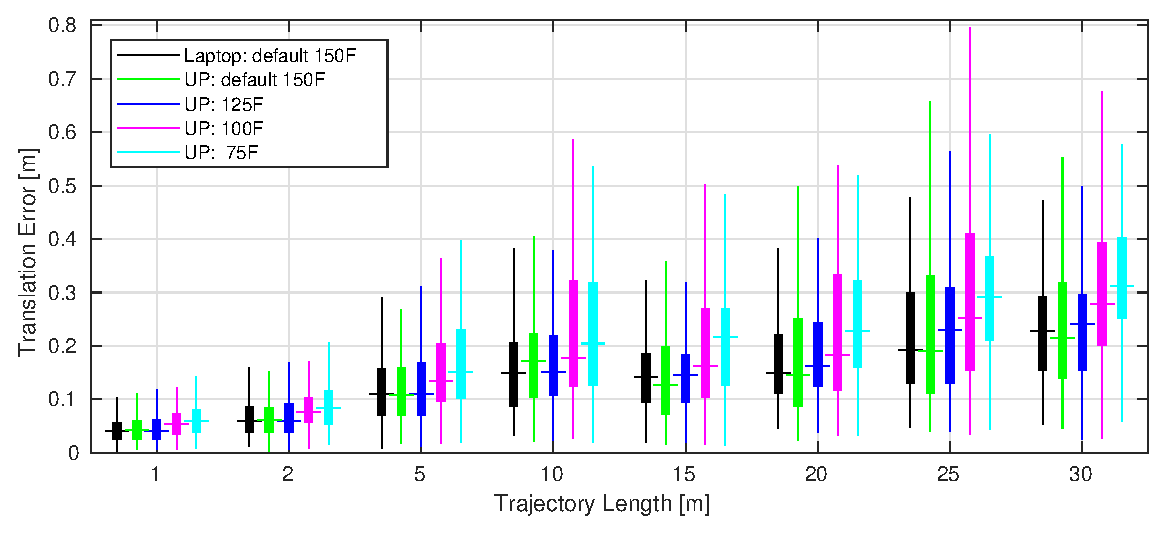
\includegraphics[width=0.95\textwidth]{images/acc_features}
\caption{Boxplot summarizing the translation error statistic for the \ac{VIO} 
pipeline when changing the number of tracked features over consecutive frames.  
The analyzed number of tracked features are \{150, 125, 100, 75\}. The first 
number is the default setting and is evaluated on a Laptop and on a UP Board, 
all other numbers are evaluated on a UP Board. Errors were computed using the 
metric described in \autoref{subsec:accuracy} for trajectory segments of length 
\{1,2,5,10,15,20,25,30\} m.}
\label{fig:acc_feature}
\end{figure}


\section{Changing the Sliding Window Size}\label{sec:slidingWindow}
The non-linear \ac{BA} is performed over a sliding window containing the latest 
two frames and a number of previous keyframes. The default window size is 10, 
which means that the number of previous keyframes is eight. In this section the 
impact of the window size is analyzed. 

The reduction in the number of keyframes has influence on the optimization and 
the marginalization. With less keyframes, the number of poses in the ``pose 
block'' $\vec{\Lambda}_{p}$ in Equation \eqref{eq:system} is reduced, as every 
keyframe leads to a pose. Also the number of corresponding landmark observations 
in the keyframes is potentially reduced. For an alternative explanation we can 
take a closer look at the dimensions of the system matrix in Equation 
\eqref{eq:system}. With a reduced number of poses, the dimensions of the 
symmetric ``pose block'' $\vec{\Lambda}_{p}$ is reduced. Therefore, the number 
of columns of the ``observation block'' $\vec{\Lambda}_{mp}$ has to be reduced 
as well. This also results in a reduced system for marginalization. The 
resulting decreased optimization times are shown in \autoref{fig:time_window}.

Furthermore, a smaller window size reduces the freely adjustable parameters in 
the optimization. The solver can then perform more iterations in the given 
limited solving time. The increased number of iterations results in a higher 
convergence rate, which counteracts the decreased accuracy due to the smaller 
window size. Because of this, the translation error does not increase much 
along the different window sizes as seen in \autoref{fig:acc_window}.
\begin{figure}[H]
\centering
\includegraphics[width=1\textwidth]{images/time_window}
\caption{Boxplot summarizing the whole optimization time (optimization and 
marginalization) for the \ac{VIO} pipeline when changing number of keyframes in 
the sliding window. The analyzed number of keyframes in the window are \{$8, 6, 
4, 2$\}, which results together with the latest two frames in a window size of 
\{$10, 8, 6, 4$\}. The first number is the default setting and is evaluated on 
a Laptop and on a UP Board, all other numbers are evaluated on a UP Board.  
The average numbers of solver iterations for the five 
different cases are \{$6.00, 2.06, 2.69, 3.21, 4.73$\} iterations.}
\label{fig:time_window}
\end{figure}
\begin{figure}[H]
\centering
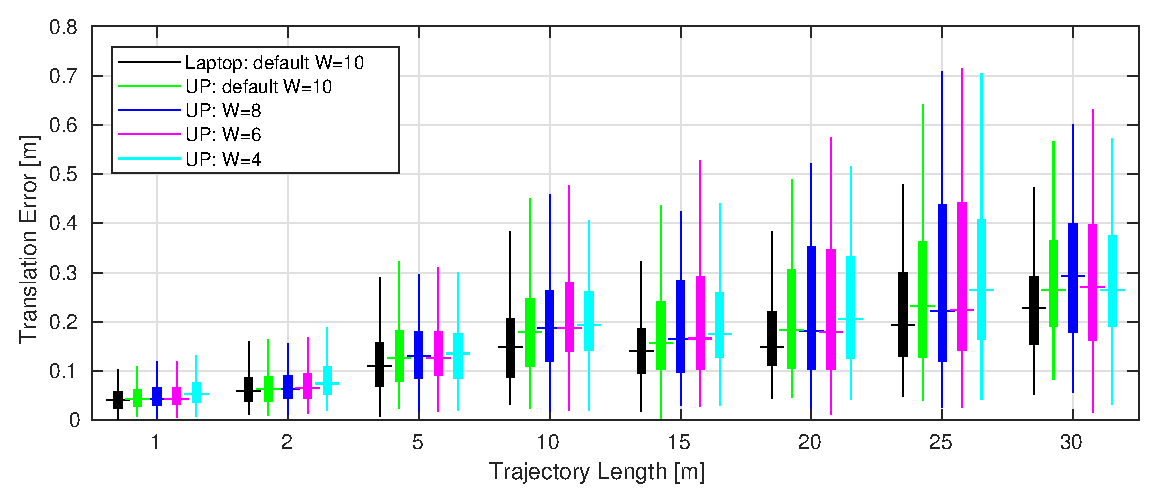
\includegraphics[width=1\textwidth]{images/acc_window}
\caption{Boxplot summarizing the translation error statistic for the \ac{VIO}
pipeline when changing number of keyframes in the sliding window. The tested 
number of keyframes in the window are \{$8, 6, 4, 2$\}, which results together 
with the latest two frames in a window size of \{$10, 8, 6, 4$\}. The first 
number is the default setting and is evaluated on a Laptop and on a UP Board, 
all other numbers are evaluated on a UP Board. 
Errors were computed using the metric described in \autoref{subsec:accuracy} 
for trajectory segments of length \{$1, 2, 5, 10, 15, 20, 25, 30$\} m. }
\label{fig:acc_window}
\end{figure}

\section{Setting Features Constant in Optimization} \label{sec:constFeatures}
Another method to reduce the number of freely adjustable variables in the 
optimization is to set the constraints of landmarks observed in the oldest 
keyframes in the window to constants. The idea behind this approach is, that 
the features corresponding to these landmarks have already been optimized 
several times. The constraints of these features are added as residuals, but 
will not change during the optimization. 
The resulting changes in per-frame optimization time and accuracy can be seen 
in \autoref{fig:time_const} and \autoref{fig:acc_const}, respectively. This 
approach has almost no effect on the overall optimization time. The entries in 
the system matrix stay the same and hence, the number of factors in the 
marginalization does not change either. One can see a significant decrease in 
accuracy for this approach. The reason is assumed to be the method how VINS-Mono 
represents the features. They are not represented as a position in the 3D map 
but as a single parameter, the inverse depth. This means, setting the inverse 
depth constant restricts much more than setting the feature position constant.
\begin{figure}[H]
\centering
\includegraphics[width=1\textwidth]{images/time_const}
\caption{Boxplot summarizing the whole optimization time (optimization and 
marginalization) for the \ac{VIO} pipeline when setting the feature constraints 
as constants in the \ac{BA} optimization for a number of oldest keyframes in the 
sliding window. The analyzed numbers of oldest keyframes are \{$0, 2, 4, 6$\} 
corresponding to the keyframe position \{none, KF $7\!-\!8$, KF $5\!-\!8$, KF 
$3\!-\!8$\}. The default setting is evaluated on a Laptop and a UP Board. The 
different number of keyframes, where the feature constraints are constant, is 
evaluated on a UP Board. The average numbers of solver iterations for the five 
different cases are \{$6.00, 2.06, 2.56, 2.66, 2.73$\} iterations.}
\label{fig:time_const}
\end{figure}
\begin{figure}[H]
\centering
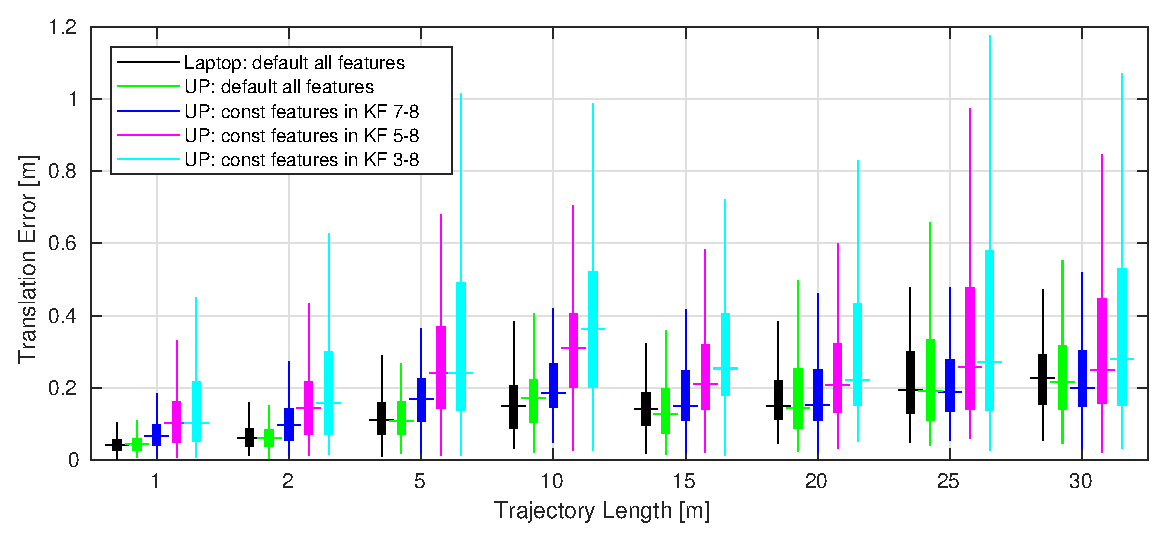
\includegraphics[width=1\textwidth]{images/acc_const}
\caption{Boxplot summarizing the translation error statistic for the \ac{VIO}
pipeline when setting the constraints as constants in the \ac{BA} from the 
features observed in the oldest keyframes in the sliding window. The 
analyzed numbers of oldest keyframes are \{$0, 2, 4, 6$\} corresponding to the 
keyframe position \{none, KF $7\!-\!8$, KF $5\!-\!8$, KF $3\!-\!8$\}. The 
default setting is evaluated on a Laptop and a UP Board. The different number 
of keyframes, where the feature constraints are constant, is evaluated on a UP 
Board. Errors were 
computed using the metric described in \autoref{subsec:accuracy} for trajectory 
segments of length \{$1, 2, 5, 10, 15, 20, 25, 30$\} m.}
\label{fig:acc_const}
\end{figure}

\begin{minipage}[b]{1\linewidth}
\section{Not adding Features of the oldest Keyframes to the Bundle Adjustment} 
\label{sec:dontOptimizeOldest}
A similar adaptation as changing the window size is as follows. For a number of 
old keyframes in the window we do not add any feature constraints. This is 
equal to reducing the optimization to a pose graph optimization for these 
keyframes.

Due to the implementation of VINS-Mono, the marginalization is not 
affected by this change since the system matrix in Equation \eqref{eq:system} is 
created independently of the parameters the optimization is performed on. As 
shown in \autoref{fig:time_continue_oldest} 
the per-frame optimization time decreases only slightly. The translation error 
increases only barely, as shown in \autoref{fig:acc_continue_oldest}.
This implies that the constraints from 
features do not have as much influence in the older keyframes as they have in 
the newer (key-)frames. The reason is, that the older keyframes have already 
been optimized several times when they reach the end of the sliding window. 
\begin{figure}[H]
\centering
\includegraphics[width=1\textwidth]{images/time_continue_oldest}
\caption{Boxplot summarizing the whole optimization time (optimization and 
marginalization) for the \ac{VIO} pipeline when ignoring the feature 
constraints in the \ac{BA} optimization in a number of oldest keyframes in the 
sliding window. The analyzed numbers of oldest keyframes in which no feature 
constraints are added are \{$0, 2, 4, 6$\} corresponding to the keyframe 
position \{none, KF $7\!-\!8$, KF $5\!-\!8$, KF $3\!-\!8$\}. The default 
setting is evaluated on a Laptop and a UP Board. The different number of 
keyframes where the feature constraints are ignored are evaluated on a UP 
Board. The average numbers of solver iterations for the five different cases are 
\{$6.00, 2.06, 2.17, 3.09, 3.10$\} iterations.}
\label{fig:time_continue_oldest}
\end{figure}
\begin{figure}[H]
\centering
\includegraphics[width=1\textwidth]{images/acc_continue_oldest}
\caption{Boxplot summarizing the translation error statistic for the \ac{VIO}
pipeline when ignoring the feature 
constraints in the \ac{BA} optimization in a number of oldest keyframes in the 
sliding window. The analyzed numbers of oldest keyframes in which no feature 
constraints are added are \{$0, 2, 4, 6$\} corresponding to the keyframe 
position \{none, KF $7\!-\!8$, KF $5\!-\!8$, KF $3\!-\!8$\}. The default 
setting is evaluated on a Laptop and a UP Board. The different number of 
keyframes where the feature constraints are ignored are evaluated on a UP 
Board. Errors were computed using the metric described in 
\autoref{subsec:accuracy} for trajectory segments 
of length \{$1, 2, 5, 10, 15, 20, 25, 30$\} m.}
\label{fig:acc_continue_oldest}
\end{figure}
\end{minipage}


\begin{minipage}[b]{1\linewidth}
\section{Removing Features from the Bundle Adjustment} \label{sec:dontOptimize}
We looked for other ways to reduce the number of parameters the optimization is 
performed on. A similar but more radical approach as the one described before 
is ignoring landmarks, which are observed in at least one of 
the oldest keyframes in the sliding window, in all (key-)frames in the \ac{BA} 
optimization. This allows the solver to perform more iterations in the given 
solving time similar to the approach of reducing the sliding window size. As in 
the previous approach, the marginalization is not affected by this change. The 
effect on the optimization time is almost negligible, as shown in 
\autoref{fig:time_continue}. However, if too many landmarks are ignored, the 
translation error increases noticeably, as shown in  
\autoref{fig:acc_continue}. Otherwise, the accuracy is affected only slightly.
\begin{figure}[H]
\centering
\includegraphics[width=1\textwidth]{images/time_continue}
\caption{Boxplot summarizing the whole optimization time for the \ac{VIO} 
pipeline when ignoring the feature constraints in the \ac{BA} optimization in 
all (key-)frames if the feature has been observed in one of a number of oldest 
keyframes in the sliding window. The analyzed numbers of oldest keyframes, in 
which no feature constraints are added, are \{$0, 2, 4, 6$\} corresponding to 
the keyframe position \{none, KF $7\!-\!8$, KF $5\!-\!8$, KF $3\!-\!8$\}. The 
default setting is evaluated on a Laptop and a UP Board. The different number 
of old keyframes, which decide if a feature constraints, is ignored in all 
(key-)frames is evaluated on a UP Board. The average numbers of solver 
iterations for the five different cases are \{$6.00, 2.06, 4.72, 5.37, 6.78$\} 
iterations.}
\label{fig:time_continue}
\end{figure}
\begin{figure}[H]
\centering
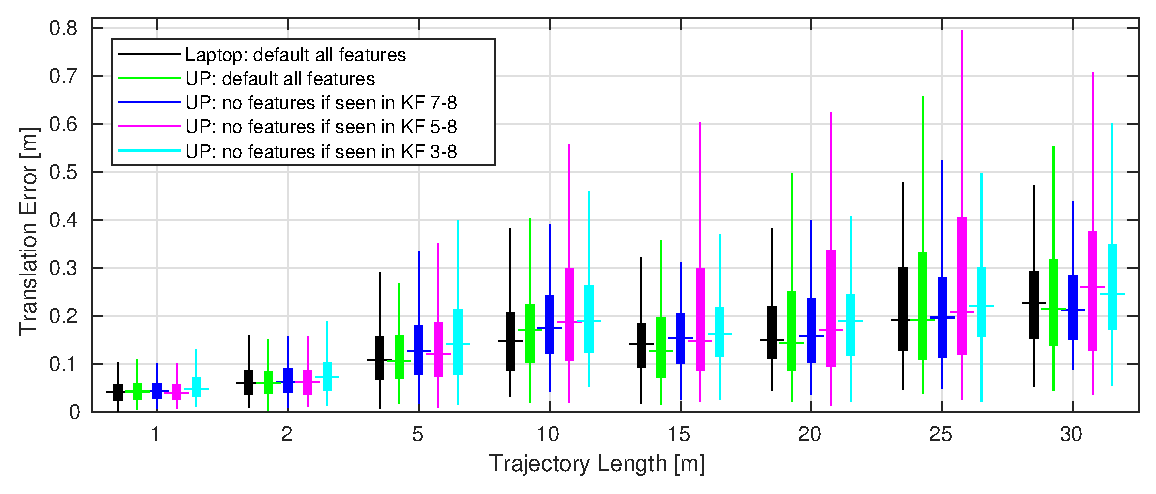
\includegraphics[width=1\textwidth]{images/acc_continue}
\caption{Boxplot summarizing the translation error statistic for the \ac{VIO}
pipeline when ignoring the feature constraints in the \ac{BA} optimization in 
all (key-)frames if the feature has been observed in one of a number of oldest 
keyframes in the sliding window. The analyzed numbers of oldest keyframes, in 
which no feature constraints are added, are \{$0, 2, 4, 6$\} corresponding to 
the keyframe position \{none, KF $7\!-\!8$, KF $5\!-\!8$, KF $3\!-\!8$\}. The 
default setting is evaluated on a Laptop and a UP Board. The different number 
of old keyframes, which decide if a feature constraints, is ignored in all 
(key-)frames is evaluated on a UP Board. Errors were computed using the metric 
described in \autoref{subsec:accuracy} for trajectory segments of length 
\{$1, 2, 5, 10, 15, 20, 25, 30$\} m.}
\label{fig:acc_continue}
\end{figure}
\end{minipage}

\section{Skipping Marginalization} \label{sec:dontMarginalize}
This evaluations focuses on the marginalization. The effect of ignoring the 
marginalization fully can be seen in \autoref{fig:time_no_marginalize} and 
\autoref{fig:acc_no_marginalize}. We can see that the overall optimization 
time is drastically reduced, confirming that the marginalization is responsible 
 for the increased timing on the UP Board. However, we can also see that the 
accuracy is reduced drastically, implying that ignoring the marginalization is 
not an option. 
\begin{figure}[H]
\centering
\includegraphics[width=1\textwidth]{images/time_no_marginalize}
\caption{Boxplot summarizing the whole optimization time (optimization and 
marginalization) for the \ac{VIO} pipeline when marginalization is performed 
compared to no marginalization. The default marginalization is evaluated on a 
Laptop and on a UP Board and no marginalization is evaluated on a UP Board. The 
average numbers of solver iterations for the three different cases are \{$6.00, 
2.06, 2.30$\} iterations.}
\label{fig:time_no_marginalize}
\end{figure}
\begin{figure}[H]
\centering
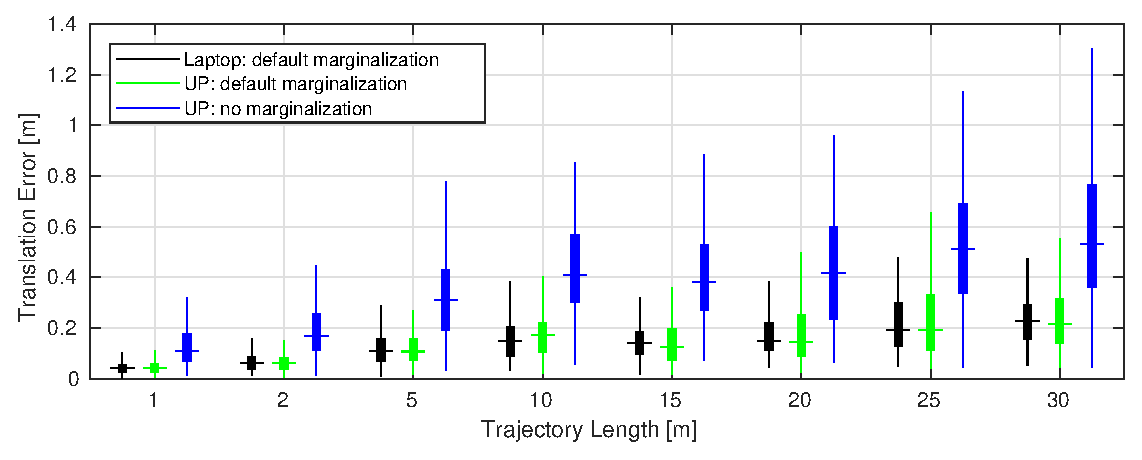
\includegraphics[width=1\textwidth]{images/acc_no_marginalize}
\caption{Boxplot summarizing the translation error statistic for the \ac{VIO}
pipeline when marginalization is performed compared to no marginalization. The 
default marginalization is evaluated on a Laptop and on a UP Board and no 
marginalization is evaluated on a UP Board. Errors were computed using the 
metric described in \autoref{subsec:accuracy} for trajectory segments of length 
\{$1, 2, 5, 10, 15, 20, 25, 30$\} m.}
\label{fig:acc_no_marginalize}
\end{figure}

\section{Removing Features from Marginalization}\label{sec:remove_marginalize}
To reduce the number of parameters in the marginalization the following 
approach was analyzed. Features are only marginalized if their 
corresponding landmarks have been observed in more than a certain number of 
keyframes. This reduces the dimensions of the system matrix in Equation 
\eqref{eq:system}, leading to a reduced marginalization time as shown in 
\autoref{fig:time_marginalize}. 

Reducing the parameters in the marginalization has also impact on the prior in 
the non-linear \ac{BA}. A prior is only added for features that have been 
marginalized, which implicitly reduces the freely adjustable parameters in the 
optimization. This again allows for more iterations in the same solving time. If 
only landmarks observed in more than two keyframes are marginalized the 
translation error decreases. However, if too many landmarks are ignored in the
marginalization the absence of the corresponding prior in the \ac{BA} 
optimization leads to increased translation errors. These effects are shown in 
\autoref{fig:acc_marginalize}.
\begin{figure}[H]
\centering
\includegraphics[width=1\textwidth]{images/time_marginalize}
\caption{Boxplot summarizing the whole optimization time (optimization and 
marginalization) for the \ac{VIO} pipeline when only marginalize features if 
their corresponding landmarks have been observed in a minimum 
number of (key-)frames in the sliding window. The analyzed numbers of 
(key-)frames are \{$0, 2, 4, 6$\}. The default setting is evaluated on a Laptop 
and a UP Board. The minimum number of (key-)frames a landmark has to be 
observed in is evaluated on a UP Board. The average numbers of solver 
iterations for the five different cases are \{$6.00, 2.06, 2.15, 2.15, 2.14$\} 
iterations.}
\label{fig:time_marginalize}
\end{figure}
\begin{figure}[H]
\centering
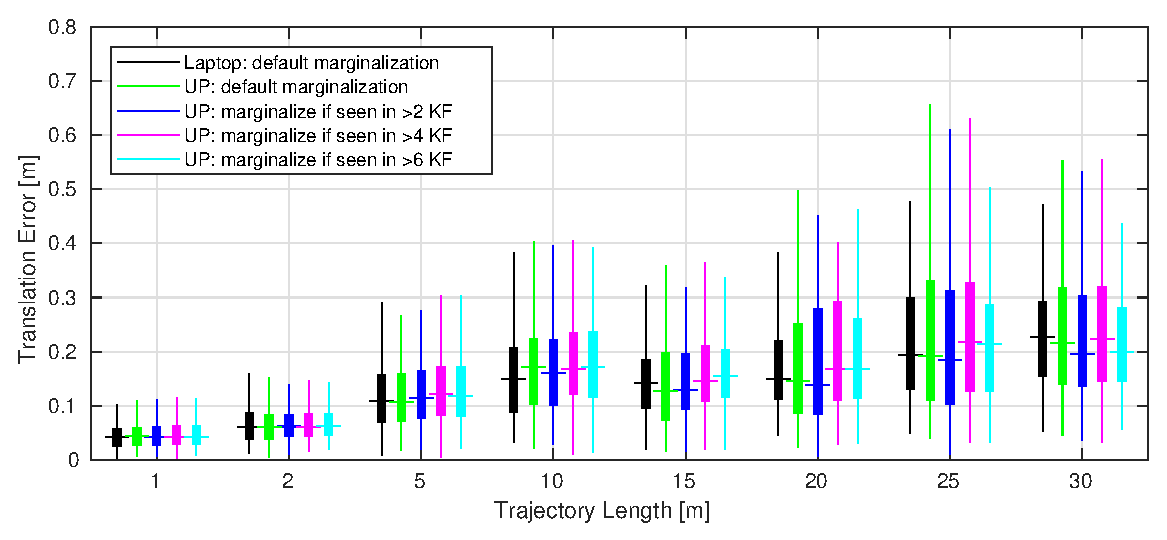
\includegraphics[width=1\textwidth]{images/acc_marginalize}
\caption{Boxplot summarizing the translation error statistic for the \ac{VIO}
pipeline when only marginalize features if their corresponding landmarks have 
been observed in a minimum 
number of (key-)frames in the sliding window. The analyzed numbers of 
(key-)frames are \{$0, 2, 4, 6$\}. The default setting is evaluated on a Laptop 
and a UP Board. The minimum number of (key-)frames a landmark has to be 
observed in is evaluated on a UP Board. Errors were computed 
using the metric described in \autoref{subsec:accuracy} 
for trajectory segments of length \{$1, 2, 5, 10, 15, 20, 25, 30$\} m.}
\label{fig:acc_marginalize}
\end{figure} 
\newpage

\section{Conclusion}\label{sec:eval_conclusion}
As mentioned in the beginning of this chapter, the overall optimization time 
consists of the time to solve the \ac{BA} 
optimization and the time needed for the marginalization.

A first setting to reduce the overall optimization time is to limit the number 
of tracked features. 

The maximal time the 
solver can spend for the \ac{BA} optimization is fixed and in most of the cases 
the termination criteria of the 
optimization. Therefore, reducing the number of parameters the optimization is 
performed on does not decrease the optimization time but increases the number 
of iterations the optimizer can perform in the given solving time, which 
results in an increased accuracy.

The best way to decrease the number of parameters, the \ac{BA} optimization has 
to optimize, while still achieving a reasonable accuracy is the approach 
presented in \autoref{sec:dontOptimize}.

The best trade off between time and accuracy for marginalization achieved the 
approach in which only landmarks are marginalized which were observed in more 
than a certain number of keyframes described in 
\autoref{sec:remove_marginalize}.

Based on these insights from the evaluation, we build our proposed approach, 
presented in the next chapter.